\item \subquestionpointscoding{2}
Follow the instructions in \texttt{linearclass/src/logreg.py} to train a logistic regression classifier using Newton's Method. Starting with $\theta = \vec{0}$, run Newton's Method until the updates to $\theta$ are small: Specifically,  train until the first iteration $k$ such that $\|\theta_{k} - \theta_{k-1}\|_1 < \epsilon$, where $\epsilon = 1\times 10^{-5}$. Make sure to write your model's predicted probabilities on the validation set to the file specified in the code.

To verify a correct implementation, consider creating a plot of the \textbf{validation data} with $x_1$ on the horizontal axis and $x_2$ on the vertical axis. To visualize the two classes, use a different symbol for examples $x^{(i)}$ with $y^{(i)} = 0$ than for those with $y^{(i)} = 1$. On the same figure, plot the decision boundary found by logistic regression (i.e, line corresponding to $p(y|x) = 0.5$).

Your plot should look similar to the following:

\begin{figure}[H]
	\centering
	\vspace{2mm}
	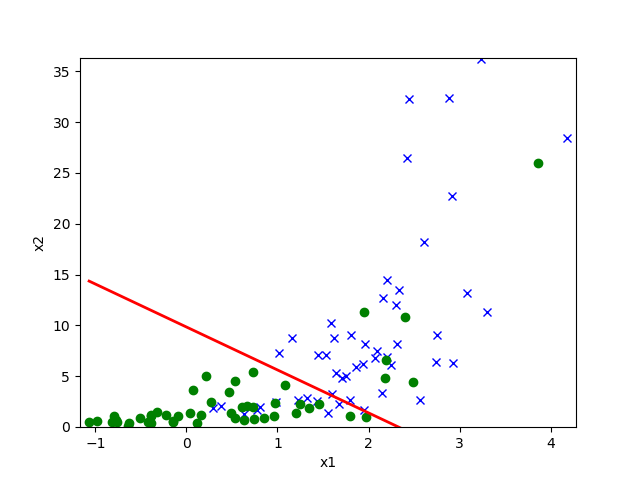
\includegraphics[width=0.65\linewidth]{linearclass/src/p01b_pred_1.png}
    \caption{Separating hyperplane for logistic regression on Dataset 1}
\end{figure}
